% Chapter 1

\chapter{Introduction} % Main chapter title
\PartialToc

\label{Chapter1} % For referencing the chapter elsewhere, use \ref{Chapter1} 

%----------------------------------------------------------------------------------------

% Define some commands to keep the formatting separated from the content 
\newcommand{\keyword}[1]{\textbf{#1}}
\newcommand{\tabhead}[1]{\textbf{#1}}
\newcommand{\code}[1]{\texttt{#1}}
\newcommand{\file}[1]{\texttt{\bfseries#1}}
\newcommand{\option}[1]{\texttt{\itshape#1}}

%----------------------------------------------------------------------------------------

Si la connaissance de la couverture de la surface terrestre a historiquement été importante pour des raisons sociales et économiques, celle-ci est également devenue fortement liée aujourd'hui aux préoccupations en matière d'environnement et de climat. Les changements globaux en jeu sont visibles à la surface de la Terre, que ceux-ci soient anthropiques ou bien naturels.\\
L'observation à large échelle des dynamiques continentales s'avère donc cruciale. Les capteurs spatiaux d'observation de la Terre répondent à ce besoin au travers de données images à différentes résolutions spatiales et spectrales. Cette source de données quasi continue permet de donner matière à des processus de cartographie du sol.\\
Dans un monde où les changements sont très rapides, il est dorénavant essentiel de cartographier à une fréquence soutenu le paysage. Or, les capteurs fournissant énormément de données à analyser, il devient ardu de répondre à cela par des moyens purement manuels. C'est pourquoi les communautés scientifiques se tournent vers des processus automatiques : en particulier, les algorithmes d'apprentissage profonds ont démontré leur efficacité dans de nombreux domaines et se révèlent prometteurs en matière de cartographie des sols.\\
Après avoir défini le terme d'occupation des sols et passé en revu les différents produits existants, un état des capteurs dédiés à l'observation de la Terre est réalisé. D'un point de vue méthodologique, on explicite pourquoi l'approche par apprentissage profond a été retenue et les travaux existants en faisant usage. Enfin, la problématique de la thèse ainsi que ses tenants et aboutissants sont explicités en fin de chapitre.
%%%%%%%%%%%%%%%%%%%%%%%%%% SECTION 1 %%%%%%%%%%%%%%%%%%%%%%%%%%
\section{Cartographie de l'occupation des sols}
\label{sec:ocs}
La définition que l'on peut donner de l'occupation des sols est la suivante : il s'agit de la description physique de l'ensemble de la surface terrestre selon une nomenclature donnée ; on considère donc par ce terme aussi bien les surfaces anthropiques que naturelles.\\
Cette description est à différencier de l'usage du sol qui traduit la fonction sociale ou économique exercée par l'objet présent sur l'occupation des sols. Pour illustrer la différence entre les deux cartographies en milieu urbain, là où l'occupation intègre généralement une classe unique \textit{bâti}, l'usage, quant à elle, distingue au sein de cette classe les bâtiments à caractère commercial ou bien industriel. L'utilisation seule d'images satellite pour la classification du sol rend ardue la détection de classes d'usage du sol. En effet, l'analyse purement de la radiométrie ne permet pas de représenter de telles classes dont les définitions reposent purement sur des considérations sociales ou économiques. Occupation et usage sont souvent mêlées au sein de bases de données existantes : par exemple, Corine Land Cover, base de données établie à l'initiative de l'Agence européenne pour l'environnement (AAE), regroupe aussi bien des classes d'occupation telles que \textit{Forêts et milieux semi-naturels} et \textit{Surface en eau}, que des des classes d'usages telles que \textit{Zones industrielles ou commerciales et installations publiques}.\\
Outils aussi bien scientifiques que décisionnels, les cartes d'occupation des sols fournissent une description utile et nécessaire à la compréhension et au suivi de phénomènes naturels ou anthropiques. Elles constituent une base de travail indispensable à des organismes comme le GIEC (\textit{Groupe d'experts intergouvernemental sur l'évolution du climat}), notamment sur la question du stockage du carbone dans le sol et dans les arbres, et le problème posé par la déforestation (libération du carbone dans l'atmosphère). La connaissance de la nature du sol à différentes dates guide la prise de mesures et la gouvernance à adopter dans un contexte où les changements climatiques sont globaux, en témoigne le rapport de la Cour des Comptes de 2012 \citep{cc2018}, dans lequel il est révélé que la réaffectation des sols et le défrichement pour la production de biocarburants conduit finalement à une augmentation d'émissions de gaz à effet de serre plus importantes que celles issues d'énergies hydrocarbures (en plus de soustraire une partie de la surface totale des terres arables à destination alimentaire). En terme de gestion des risques liés à l'environnement, la cartographie des sols joue un rôle crucial (prévention, simulation, acheminement de secours) : par exemple, les surfaces inondables, en croissance continue due au réchauffement climatique global et à la montée des eaux, les forêts susceptibles de subir un incendie, ou encore les zones d'avalanche sont référencées et disponibles en France grâce à l'outil mis en place en juillet 2014 par le Ministère de l'Ecologie, du Développement durable et de l'Energie et le BRGM (Bureau de recherches géologiques et minières) \footnote{http://www.georisques.gouv.fr/cartes-interactives}, suite à la tempête Xynthia de 2010.\\
En matière d'urbanisme et politiques territoriales en France, des documents tels que les Plans Locaux d'Urbanisme (PLU), Schémas de Cohérence Territoriale (SCoT) s'appuient sur la connaissance de l'occcupation des sols. En particulier, l'étalement urbain et l'imperméabilisation croissante des sols sont des sujets sur lesquels la législation a imposé des limites, afin de préserver les zones naturelles et les surfaces agricoles utiles ; à cette fin la Loi d'avenir pour l'agriculture, l'alimentation et la forêt met notamment en place au niveau départemental une commission de la préservation des espaces naturels, agricoles et forestiers \footnote{Loi \no 2014-1170 du 13 octobre 2014 d'avenir pour l'agriculture, l'alimentation et la forêt} qui émet des avis lors de l'élaboration de PLU et SCoT, au regard d'un objectif de préservation des terres agricoles et naturelles.\\
La connaissance de l'occupation des sols étant donc essentielle pour de nombreux usages, il convient pour chacun d'entre eux de fournir l'outil adéquat. Pour cela, les cartes d'occupation sont caractérisées par plusieurs spécifications détaillés en première partie. En seconde partie, un panel de cartographies existantes ou en cours d'élaboration sera présenté et



\subsection{Caractérisation d'une carte d'occupation des sols}
\label{ssec:carac_ocs}
Un certain nombre de caractéristiques permettent de décrire une carte d'occupation des sols d'un point de vue méthodologique :
\begin{enumerate}
    \item la zone couverte par la couverte sur la surface terrestre (échelle locale ? globale ?)
    \item la sémantique incluant :
    \begin{itemize}[label=\textbullet]
        \item la nomenclature : les classes d'intérêt choisies pour décrire l'environnement que l'on cherche à étudier. Une nomenclature peut avoir une granularité plus ou moins fine, ce qui correspond au niveau de détail souhaité : les nomenclatures existantes adoptent bien souvent une structure hiérarchique emboîtée\footnote{on entend par hiérarchie emboîtée la notion de classes \og mères\fg{} et classes \og filles \fg{} : la classe \textit{bâti} peut être ainsi subdivisée en \textit{habitat} et \textit{bâti à usage commercial ou industriel}.};
        \item la précision de cette sémantique lorsque l'on compare les classes attribuées par rapport à la réalité observable ;
    \end{itemize}
    \item les règles géographiques :
    \begin{itemize}[label=\textbullet]
        \item la résolution spatiale si la carte est sous format raster (pixels) ou l'unité minimal de collecte dans le cas de carte vectorielle (base de données géographiques) : tout objet inférieur en surface à cette résolution ne sera pas inventorié par la carte ;
        \item la précision géométrique permettant de qualifier la localisation des objets par rapport à la réalité : cette précision est souvent conditionnée par l'étendue géographique de la carte, si celle-ci couvre le globe entier par exemple, et donc l'on privilégie une analyse statistique, la délimitation géométrique exacte des objets n'aura que peu d'importance ;
    \end{itemize}
    \item le millésime associé à la carte : pour le suivi de phénomènes temporels, il est indispensable de disposer de cartes à plusieurs dates afin de retracer leur évolution. 
\end{enumerate}

Tous ces éléments contribuent à l'élaboration du cahier des charges pour la carte d'occupation des sols souhaitée par l'utilisateur final. Si ces points peuvent apparaître triviaux, il est néanmoins nécessaire de les aborder avec rigueur car cela conditionne toute la suite du processus de cartographie d'occupation des sols. 


\subsection{Offres actuelles en OCS}
Au regard des paramètres passés en revue en \ref{ssec:carac_ocs}, différentes cartes d'occupation des sols ont déjà été produites. Nous nous restreignons aux produits englobant le territoire français afin de respecter le cadre de notre étude. \\
La \textcolor{red}{Figure -------~\ref{fig:ocs}} présente différentes cartes d'occupation, dont les caractéristiques sont ensuite détaillées carte par carte, pour la ville de Vannes, ainsi que l'image Spot de 2017 couvrant la zone. Il est visuellement possible d'apprécier un certain nombre des paramètres évoqués en \ref{ssec:carac_ocs}. Tout d'abord les différentes échelles d'information disponibles : Corine Land Cover (\textcolor{red}{carte ------~\ref{fig:ocs_clc}}) propose une classification à l'échelle de l'Europe, permettant une analyse pertinente du paysage à une échelle très globale et nationale. Cependant, une telle échelle rend difficile la description fine de la structure d'une ville ; en particulier les routes sont absentes, ayant une finesse morphologique trop importante pour rentrer dans les critères de représentation de la base de données. Pour étudier un paysage en milieu urbain dense par exemple, on préfère une carte offrant une résolution spatiale plus fine telle que proposée par l'OCS-GE (Occupation des sols à Grand Echelle) de l'IGN (Institut National de l'Information Géographique et Forestière), visible sur la \textcolor{red}{Figure ------~\ref{fig:ocs_ge}}.

%%%%%%%%%%%% OCS existantes (sur Vannes)
%%% Spot image / CLC / Urban Atlas / OSO / OCS-GE / 
\begin{figure}
    \centering
    \includegraphics{}
    \caption{Exemples de cartes d'occupation des sols existantes sur l'agglomération de la ville de Vannes, dans le Morbihan (56)}
    \label{fig:ocs_existantes}
\end{figure}

\subsubsection{Initiatives globales}
\label{sssec:glob_ocs}
A l'échelle européenne, le projet européen GMES (Global Monitoring for Environment and Security), aujourd'hui connu sous le nom Copernicus, a la charge de fournir des données d'observation de la Terre dans un objectif de surveillance. Ce programme est à l'origine de la réalisation de la base de données d'occupation des sols Corine Land Cover. Celle-ci fait également partie du champ de la directive INSPIRE (Infrastructure d'information géographique dans la Communauté européenne), et a pour but de cibler les classes prioritaires d'un point de vue environnemental, de coordonner les efforts pour la collection des données relatives à ces classes et de s'assurer la compatibilité entre toutes les données collectées par les différents organismes impliqués. Les données Corine Land Cover sont libres et gratuites d'accès.\\
Corine Land Cover couvre 39 pays d'Europe - Union Européenne et pays limitrophes (\textcolor{red}{Figure ---------~\ref{fig:clc_europe}}) - et est produite manuellement par photo-interprétation d'images satellites de 20 à 25 mètres de résolution, afin de répertorier les objets ayant une surface (Unité Minimale de Collecte - UMC) de 25 hectares. Quatre millésimes ont été produits jusqu'à aujourd'hui : en 1990, 2000, 2006 et 2012. Les produits ultérieurs à 1990 s'accompagnent de cartes de changements entre deux itérations successives. Une nouvelle itération du produit est prévue pour fin 2018. Mêlant occupations et usages des sols, la nomenclature est hiérarchique comportant trois niveaux de détail, pour un total de 44 classes sur le niveau le plus riche, regroupées en cinq grands types d'occupation du territoire : \textit{Territoires artificialisés}, \textit{Territoires agricoles}, \textit{Forêts et milieux semi-naturels}, \textit{Zones humides} et \textit{Surfaces en eau}. Avec une UMC de 25 hectares, l'échelle d'utilisation de la base de données Corine Land Cover avoisine typiquement 1:100 000 et permet des analyses du territoire à un niveau européen, national ou régional. L'UMC contraint l'absence du réseau routier de la base de données, limitant fortement les possibilités d'utilisation en milieu urbain.\\
Si Corine Land Cover ne fournit pas de détails suffisants à l'échelle urbaine, le programme Copernicus met à disposition un second produit dédié à l'analyse urbaine appelé Urban Atlas. Il en existe deux versions, présentant toutes deux une UMC de 0,25 hectare, l'une produite en 2006, la seconde en 2012. Cette base de données est disponible sur toute l'Europe mais de façon localisée (discontinue). En effet, si l'on considère la version de 2012, seules les agglomérations de plus de 50 000 habitants y sont référencées, pour un total de 697 unités urbaines. La description urbaine fine, visible sur la \textcolor{red}{Figure ---------~\ref{fig:ocs_UA}}.

%%%%%%%% CLC
\begin{figure}
    \centering
    \includegraphics{}
    \caption{Couverture de la base de données européennes d'occupation des sols Corine Land Cover en 2012.}
    \label{fig:clc_europe}
\end{figure}

\subsubsection{Initiatives nationales}
\label{sssec:nat_ocs}
De multiples projets d'occupation des sols existent en France, et sont plus ou moins aboutis. Chacun d'entre eux répond généralement à un besoin local à court terme. Quelques exemples seront évoqués dans la partie suivante (Section~\ref{sssec:loc_ocs}). Même si ceux-ci restent pertinents dans un contexte régionale, voire à une échelle plus petite encore, l'étude de certaines thématiques nationales telles que le parc forestier ou l'artificialisation des sols en France nécessite des cartes d'occupation des sols homogènes sur le territoire, tant au niveau de la nomenclature, que des processus de production mis en \oe{} pour construire ces cartes. A cette fin, le pôle de données et de services surfaces continentales  Theia a initié, au travers du Centre d'Expertise Scientifique (CES) Occupation des SOls (OSO)\cite{inglada2017} porté par le Centre d'Etudes Spatiales de la BIOsphère (CESBIO), la production automatique de cartes annuelles d'occupations des sols à l'échelle de la France entière. L'utilisation de séries temporelles Sentinel-2 dans un processus de classification supervisée permet notamment de discriminer efficacement en milieu naturel les différentes essences forestières ou encore le type de culture en présence. Le but de ce CES est de proposer chaque année une nouvelle carte d'occupation calculée sur les données satellites acquises l'année précédente. Ainsi, la première carte disponible pour la France entière a été mise à disposition début 2017, et produite à partir des données récoltées en 2016 par les deux satellites Sentinel-2 (\textcolor{red}{Figure~\ref{fig:oso}}). La carte résultante comporte entre 14 et 17 classes selon la nomenclature adoptée en milieu urbain, et est disponible avec une résolution à (i) \SI{20}{\meter} nativement ou (ii) \SI{10}{\meter} après sur-échantillonnage. Une seconde carte a été mise à disposition début 2018, après classification des séries temporelles acquises en 2017.\\
De son côté, l'Institut National de l'Information Géographique et Forestière (IGN) a pour mission l'élaboration d'une référence nationale unique sur la France entière. Depuis 2013, cette référence est définie par des acteurs nationaux mais aussi régionaux pour répondre aux besoins locaux également, notamment en terme de compatibilité avec les nomenclature présentes sur les cartes d'occupations locales. Cette référence répond aussi au besoin de conformité avec la directive INSPIRE. En plus, des spécifications supplémentaires contraignent davantage cette référence : l'adéquation avec le Référentiel Grande Echelle (RGE) de l'IGN qui rassemble diverses couches de données (BD Ortho, BD Topo, BD Adresse, BD Parcellaire, RGE Alti), une précision suffisante pour permettre son utilisation à une échelle locale (cohérence spatiale avec les SCoTs), une fréquence de mise à jour régulière et rapide. A ces fin, l'IGN a établi une nomenclature prenant en compte les attentes mentionnées précédemment: l'occupation des sols à grande échelle, ou OCS-GE, visible sur Figure~\ref{fig:ocs_existantes}. La nomenclature ainsi constituée s'étire sur quatre dimensions distinctes et séparées les unes des autres : occupation des sols, usages des sols, attributs morphologiques et éléments de caractérisation. Avec une granularité sémantique proposant 24 classes au niveau le plus fin, l'OCS-GE est également compatible avec Corine Land Cover. Elle est générée en deux temps :
\begin{enumerate}
    \item différentes bases de données sont superposées pour produire une première ébauche de la carte. A titre d'exemple, routes, bâtiments, réseau hydrologique sont extraits de la BD TOPO\textregistered, les forêts de la BD Forêt\textregistered, et les cultures du Registre Parcellaire Graphique (RPG). Ce processus d'extraction des bases de données permet une automatisation partielle de la production.
    \item afin de combler les vides laissés par les bases de données utilisés à l'étape précédente, un travail de photo-interprétation manuelle est exécuté sur les images de la BD ORTHO\textregistered. Il s'agit également ici de corriger les erreurs liées aux bases de données qui n'ont pas nécessairement intégré des changements récents sur l'occupation. Cette étape, bien que nécessaire, est coûteuse à la fois en temps de traitement et en opérateurs humains mobilisés.
\end{enumerate}
Il existe trois UMC pour les objets recensés dans l'OCS-GE : (i) 0.02 hectare pour les zones bâties, (ii) 0.05 hectare pour les zones construites mais non bâties (réseaux routiers, parking, réseaux ferrés...), (iii) 0.25 hectare pour les zones non construites (forêts, surfaces d'eau, parcelles agricoles...).

%%%%%%%% OSO
\begin{figure}
    \centering
    \includegraphics{}
    \caption{Carte d'occupation des sols de 2017, calculées avec des images Sentinel-2 acquises en 2016, dans le cadre du CES OSO.}
    \label{fig:oso}
\end{figure}

\subsubsection{Initiatives locales}
\label{sssec:loc_ocs}
%----------------------------------------------------------------------------------------

%%%%%%%%%%%%%%%%%%%%%%%%%% SECTION 2 %%%%%%%%%%%%%%%%%%%%%%%%%%
\section{Capteurs THRS : une opportunité pour l'OCS}
\label{sec:capteurs}
Auparavant étroitement liés aux activités militaires, les capteurs satellites acquièrent des données aujourd'hui indispensables dans la société qui est la nôtre. Du positionnement géodésique aux prévisions météorologiques, les capteurs embarqués en orbite autour de la Terre fournissent des mesures essentielles à l'élaboration de modèles d'évolution de divers phénomènes, et à la compréhension des écosystèmes dans lesquels nous vivons. En particulier, les capteurs de télédétection permettent d'imager de grandes régions en peu de temps. Dans le cas du problème d'occupation des sols, seuls les capteurs imageurs offrant des données sur les surfaces émergées nous intéressent.\\
Après avoir donné des clefs de compréhension concernant les caractéristiques des capteurs imageurs, un rapide recensement des capteurs satellites dans le contexte de la télédétection spatiale est effectué, avec un intérêt particulier pour les capteurs à très haute résolution spatiale, en particulier pour le couple de satellites SPOT 6 et 7 (Satellite Pour l’Observation de la Terre).

\subsection{Caractéristiques des capteurs satellites}
La télédétection spatiale consiste à analyser, dans une ou plusieurs longueurs d'onde donnée(s), la fraction de rayonnement rétrodiffusé par la surface terrestre arrivant au capteur. Cette analyse conduit ensuite à l'interprétation du signal sous forme de classification par exemple dans notre cas : le comportement variant du signal par rapport à la surface  sur laquelle il a été rétrodiffusé renseigne sur sa composition et sa nature. Ce signal est à l'origine émis par le rayonnement solaire, puis capté par un capteur dit \textit{passif}, ou un capteur dit \textit{actif} émet son propre signal et mesure la quantité ré-émise par la surface. Une conséquence de la nature des capteurs actifs est la possibilité de mesurer (i) la quantité de signal reçue par rapport à celle émise, (ii) le changement de polarisation ou non de l'onde émise. Les capteurs RaDAR (Radio Detection And Ranging) et LiDAR (Light Detection And Ranging) sont des exemples de capteurs actifs, émettant des signaux dans les longueurs d'onde radio et visible/proche-visible respectivement. L'étude se limite uniquement à l'utilisation de capteurs mesurant le rayonnement rétrodiffusé à l'origine émis par le Soleil. L'inconvénient par rapport aux capteurs actifs est la nécessité d'acquérir les données pendant la journée sur la région d'intérêt.\\
Les images acquises par les capteurs actifs stockent en chaque photosite, ou pixel, la quantité de photons rétrodiffusée par la surface imagée. On appelle cette quantité la réflectance après corrections atmosphériques (modèles de transfert radiatif prenant en compte les aérosols, l'humidité...). Cette quantité mesurée par le capteur dépend de (i) la longueur d'onde (ii) le matériau sur lequel la rétrodiffusion a lieu. Il est donc intéressant d'enrichir une image en multipliant les longueurs d'onde dans lesquelles acquérir le signal rétrodiffusé, les comportements variant selon la nature du sol et permettant de construire une signature spectrale pour chaque type d'occupation. Pour illustrer ce concept de signature, la Figure~\ref{fig:vegetation_reflectance} permet de voir les spectres de réflectance de trois types d'occupation, \textit{sol nu}, \textit{neige}, \textit{végétation}. Les bandes grises visibles sur la figure correspondent aux bandes rouge, proche-infrarouge et SWIR (Shortwave Infrared) du satellite MODIS. C'est pourquoi les capteurs embarqués sur les satellites dédiés à la télédétection sont des capteurs qualifiés de \textit{multispectraux}.\\
Outre le nombre de bandes et la largeur de ces bandes (résolution spectrale), les images ont une taille de photosite intrinsèque, décidée à la conception du capteur. Cette taille est souvent assimilée, à tort, à la résolution spatiale du capteur qui se réfère en réalité à la distance minimale entre deux objets que le capteur peut séparer. La taille des photosite contraint la taille d'objet minimale que l'on peut distinguer sur l'image. Une résolution spatiale (on utilise la définition abusive de ce terme) fine permet de distinguer davantage de détails sur la surface terrestre, mais est, à surface à imager constante, plus contraignante en terme de stockage que des images à résolution spatiale moins fine.\\
Enfin, les capteurs peuvent être différenciés selon leur période de revisite, caractérisant la capacité du capteur à imager entre deux instants immédiatement consécutifs la même région. Cet aspect non négligeable permet de mener des travaux mettant en jeu des séries temporelles d'images, qui représentent la même scène à différents instants, enrichissant cette fois, non plus spectralement, mais temporellement, les caractéristiques des objets vus au sol. Ces capteurs sont très souvent embarqués sur des satellites à orbite hélio-synchrone (un tel satellite repasse quotidiennement au dessus d'un même lieu à une heure solaire locale identique), couvrant ainsi tout le globe terrestre.


\subsection{Satellites dédiés à la télédétection terrestre}
Le premier satellite dédié à des tâches de télédétection fait partie du programme civil de la NASA (National Aeronautics and Space Administration) Landsat. Il s'agit de Landsat-1, lancé en 1972. Il permettait l'acquisition de 7 bandes spectrales à une résolution de \SI{80}{\meter}, via les capteurs embarqués \textit{Return Beam Vidicon} et \textit{Multispectral Scanner}. Six satellites lui ont succédé successivement jusqu'à Landsat-8 dernier satellite en date de ce programme, lancé en 2013. Les progrès techniques permettent à celui-ci d'accroître les performances en acquérant dans 11 bandes spectrales, à une résolution de \SI{30}{\meter} pour les bandes acquises par l'\textit{Operational Land Imager} (OLI) (utiles pour l'analyse des surfaces émergées). Ce capteur fournit des images à haute résolution, avec une période de revisite de 16 jours. Une nouvelle itération Landsat-9 est prévue pour 2020, dotée d'un capteur optique (OLI) similaire à celui de Landsat-8, mais avec une version améliorée du capteur thermique (\textit{Thermal Infrared Sensor}, ou TIRS). Ce capteur thermique est notamment utilisé pour des thématiques liées au cycle de l'eau et à la gestion de cette ressource.
Dans les années 2000, les capteurs multispectraux à faible période de revisite se sont multipliés avec tout d'abord les satellites américains Terra et Aqua, embarquant le radiomètre MODIS (\textit{Moderate Resolution Imaging Spectroradiometer}), capturant des images dans 36 bandes de \SI{0,4}{\micro\meter} à \SI{14,4}{\micro\meter}, à une résolution de \SI{250}{\meter} à \SI{1}{\kilo\meter}. Les satellites couvrent la Terre entière en 2 jours environ, et sont particulièrement attrayants pour les analyses à l'échelle mondiale liées à l'océan (chlorophylle), mais aussi au contrôle de la végétation (santé, déforestation, incendies). Toutefois, dans le but de dresser la cartographie d'occupation par des objets de dimensions pouvant approcher celles de bâtiments, ces capteurs sont inadaptés pour nos travaux. Le capteur MERIS (\textit{MEdium Resolution Imaging Spectrometer}) embarqué à bord d'Envisat, opéré par l'ESA (Agence Spatiale Européenne) et dont la mission s'est achevé en 2012, avait des spécifications techniques semblables à ceux embarquant le capteur MODIS. Le lancement de RapidEye en 2009 par l'industriel allemand éponyme, a permis la multiplication des images grâce à une constellation de 5 satellites, pour une période de revisite conjointe de 24h. L'acquisition est faite sur 5 bandes spectrales, à une résolution spatiale de \SI{5}{\meter}.\\
Plus récemment, dans le cadre du programme Copernicus, la constellation Sentinel de satellites d'observation de la Terre a été mise en place par l'ESA. Cette constellation, dont la vocation est la surveillance et le suivi de phénomènes temporels, constitue une nouveauté par (i) l'ampleur du projet, mettant en jeu divers moyens d'acquisition (actifs et passifs), (ii) la couverture du spectre électromagnétique  et (iii) la transversalité des thématiques couvertes (océans, atmosphères et terres émergées). Les satellites Sentinel-1A et Sentinel-1B\cite{TORRES20129} ont initié ce programme lors de leur lancement en 2014 et 2016, embarquant chacun un capteur RaDAR, acquérant ainsi en continu (de jour comme de nuit) mais également dans toutes les régions du globe sans difficulté (les longueurs d'onde utilisées n'étant pas ou rarement impactées par les effets atmosphériques). Ont suivi Sentinel-2A et Sentinel-2B\cite{DRUSCH201225}, lancés respectivement en 2015 et 2017, munis de capteurs optiques multispectraux : 10 bandes de \SI{10}{\meter} à \SI{20}{\meter} pour les applications d'occupation des sols, 3 bandes à \SI{60}{\meter} permettant des corrections atmosphériques et des recherches dirigées sur l'atmosphère. Le binôme Sentinel-2 offre une période de revisite de 5 jours, alliant ainsi haute fréquence temporelle, haute résolution spatiale et une couverture spectrale importante. Les données issues de ces deux satellites constituent donc une opportunité, sans précédent, très intéressante pour la cartographie de l'occupation des sols. En particulier, pour discriminer certaines classes non pérennes telles que les différents types de culture, la connaissance spectrale à différentes dates est cruciale. La troisième partie du programme, Sentinel-3\cite{DONLON201237}, est dédiée à l'étude des océans et des températures océaniques et continentales ; le premier satellite a été lancé en 2016, le second en 2018.\\

La France, en collaboration avec la Belgique et la Suède, a mis en place en 1970 le programme SPOT (Satellite Pour l'Observation de la Terre), porté par le CNES (Centre Nationale d'Etudes Spatiales). SPOT Image était propriétaire des images jusqu'en 2008, lors de son rachat par EADS Astrium. En 1986, SPOT 1 est lancé, doté d'un capteur acquérant dans 3 bandes spectrales (rouge, vert, proche-infrarouge) à \SI{20}{\meter} et d'un canal panchromatique à \SI{10}{\meter}. Ses successeurs, SPOT 2 et SPOT 3 partagent des spécifications techniques identiques que SPOT 1. SPOT 4, lancé en 1998, est également sensiblement similaire aux itérations précédentes, ajoutant toutefois une bande supplémentaire dans le moyen infrarouge. En 2002 est lancé SPOT 5, apportant une résolution spatiale accrue en proposant une image panchromatique à \SI{5}{m} et un \og supermode \fg{} permettant de produire une image à \SI{2,5}{\meter} à partir de deux images panchromatiques acquises avec un nouvel instrument, le HRG (\textit{High Resolution Geometrical}). L'acquisition superspectrale est à \SI{10}{\meter} de résolution et \SI{20}{\meter} pour la bande SWIR. Lancés en 2012 et 2014, SPOT 6 et SPOT 7 sont les deux plus récents satellites de ce programme. Les images acquises ont une résolution de \SI{6}{\meter} pour les canaux spectraux (rouge, vert, bleu, proche infrarouge) et de \SI{1,5}{\meter} pour le canal panchromatique. Les capteurs embarqués sur ces satellites sont qualifiés de capteurs à très haute résolution spatiale. En l'espace de 25 ans, la résolution a été affinée d'un facteur 6,5, offrant aujourd'hui la possibilité de cartographier des paysages difficilement discernables à des résolutions avoisinant \SI{20}{\meter}. En effet, une résolution accrue permet d'enrichir les textures des images en milieu urbain dense où il est ardu de reconnaître des patterns caractéristiques de ce paysage sur à l'aide d'image Sentinel-2. De plus, cette résolution donne accès à la détection d'objets trop fins pour d'autres capteurs, tels que les haies ou les routes. Cette nouvelle richesse sémantique est accompagnée d'une amélioration de la géométrie d'objets auxquels des capteurs à haute résolution spatiale avaient déjà accès. Les parcelles agricoles sont ainsi mieux délimitées et la mise à jour de bases de données sur ce type de classe en est facilitée. Toutefois, la très haute résolution spatiale apporte également des difficultés : la variabilité spectrale au sein d'une même classe est fortement accrue, du fait de la diversité des apparences d'objets appartenant à une même classe auxquels on a maintenant accès. En outre, le volume de données à traiter est également très lourd et limite fortement l'acquisition et le traitement de séries temporelles à cette résolution. Il est donc difficile de séparer les différents types de cultures par exemple. Pour ces raisons, des capteurs tels que ceux présents sur SPOT 6 et 7, et Sentinel-2, ne peuvent être opposés, mais sont complémentaires.


\begin{figure}
    \centering
    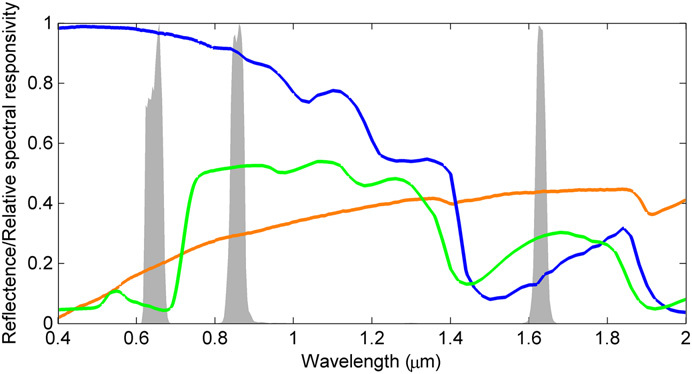
\includegraphics[scale=0.45]{Figures/chap1/vegetation_reflectance}
    \caption{Spectre de réflectance en fonction de la longueur d'onde des types de sol suivant : \textcolor{blue}{neige}, \textcolor{red}{sol nu}, \textcolor{green}{végétation}. Source\cite{wang2017rse}}
    \label{fig:vegetation_reflectance}
\end{figure}
%----------------------------------------------------------------------------------------

%%%%%%%%%%%%%%%%%%%%%%%%%% SECTION 3 %%%%%%%%%%%%%%%%%%%%%%%%%%
\section{Automatisation de la cartographie d'occupation des sols}
\label{sec:ocs_auto}
La disponibilité d'une variété très importante d'images satellites sur de très larges zones, et à des fréquences temporelles plus ou moins importantes, ouvre de nouvelles perspectives pour la description de ces zones en terme d'occupation. Les délais d'acquisition étant très brefs, les capteurs toujours actifs et détaillés notamment en \ref{sec:capteurs}, rendraient possible la mise à jour de carte d'occupation des sols existantes, ou la génération de nouvelles cartes complètes.

\subsection{Cartographie manuelle}
\label{ssec:ocs_manuelle}
Les processus de production de cartes d'occupation décrites dans la Section~\ref{sec:ocs} sont principalement manuels. Si la photo-interprétation manuelle est naïvement la plus triviale à mettre en place d'un point de vue méthodologique, elle présente plusieurs inconvénients très limitants, toutefois mitigés grâce aux protocoles de qualification et de recette rigoureux auxquels sont soumis les produits finaux.\\
Tout d'abord, il apparaît évident que les approches manuelles sont très longues, et d'autant plus longues que les surfaces à couvrir sont importantes. A titre d'exemple, les efforts à mettre en \oe{}uvre pour générer la base de données d'occupation Corine Land Cover sont tels qu'un millésime est diffusé tous les six ans depuis une vingtaine d'années, et la version calculée sur des données de 2012 n'a été diffusée qu'en 2015. Certains phénomènes lents peuvent être suivis avec une telle fréquence de mise à jour (accroissement des surfaces imperméabilisées), mais ceux-ci gagneraient de toute façon à bénéficier de versions plus rapprochées. En tout cas, beaucoup d'études ne se satisfont pas d'une telle fréquence (évolution des milieux naturels, suivi des cultures et de leurs rotations...).\\
Une limitation liée au temps de production est celle des données utilisées pour déterminer la classe d'occupation à laquelle appartient chaque objet. Un opérateur humain ne peut pas, dans les délais de production impartis, confronter différentes sources d'images (images très haute résolution spatiale, et images riches spectralement), ou bien suivre l'évolution dans le temps du comportement radiométrique de chaque objet à l'aide de séries temporelles. Cela peut générer des erreurs d'interprétation dues au manque d'information discriminante.\\
Enfin, on peut citer une source de problème inhérente au méthodes de production : diverses régions sont confiées à divers opérateurs humains, qui ont chacun leur perception des objets sur la carte, et leur expérience en matière de classification. Cela engendre une hétérogénéité spatiale qui peut également être gênante.

\subsection{Classification supervisée}
\label{ssec:cls_super}
A l'inverse des méthodes manuelles, les procédures de production automatique permettent d'utiliser diverses sources de données (ou des séries temporelles) en des temps raisonnables, tout en garantissant une homogénéité du produit puisqu'un algorithme unique est utilisé pour traiter l'ensemble des données. Ces méthodes automatiques reposent sur le concept de \textit{classification} qui consiste à attribuer à chaque pixel de l'image un label correspondant à l'une des classes de la nomenclature. Cette mécanique de classification provient de la communauté de vision par ordinateur qui s'attache en particulier à construire des méthodes toujours plus performantes de \textit{machine learning}, englobant entre autre la classification automatique. La notion de \textit{learning}, ou apprentissage, est cruciale ici et se divise en deux familles d'algorithmes : l'apprentissage supervisé et l'apprentissage non supervisé. La différence principale entre les deux familles est la connaissance \textit{a priori} (approche supervisée) ou non (approche non supervisée) des classes que l'on souhaite retrouver en fin de processus. En occupation des sols, la nomenclature a généralement été choisie au moment de l'établissement du cahier des charges de la carte souhaitée, donc en amont de la procédure de cartographie elle-même. On ne s'intéressera donc ici qu'aux méthodes de classification supervisée.\\
Reposant sur la connaissance a priori des classes, la phase d'apprentissage nécessite un \textit{jeu d'apprentissage} ou \textit{jeu d'entraînement}. Celui-ci regroupe des échantillons pour lesquels la classe d'occupation est connue. Ces échantillons peuvent être (i) des pixels ou (ii) des groupes de pixels. A partir de cette connaissance, la phase d'apprentissage permet au classifieur choisi de représenter chaque classe en fonction des échantillons lui appartenant. Afin d'obtenir cet a priori sur les classes, on extrait souvent l'information d'occupation contenue dans des bases de données géographiques (telles que celles mentionnées précédemment pour constituer l'OCS-GE).

\subsection{Essor des réseaux de neurones convolutifs}

%----------------------------------------------------------------------------------------

%%%%%%%%%%%%%%%%%%%%%%%%%% SECTION 4 %%%%%%%%%%%%%%%%%%%%%%%%%%
\section{Travail de thèse}
\subsection{Problématique}
\subsection{Stratégie proposée}
\subsection{Structure de la thèse}